\documentclass{scrartcl}

\usepackage{amssymb}
\usepackage{amsmath}
\usepackage{tikz}
\usetikzlibrary{decorations.text, arrows, arrows.meta,decorations.markings}

%both of these diagrams are from Deleuze & Guattari's Anti-Oedipus, p. 282

\begin{document}

	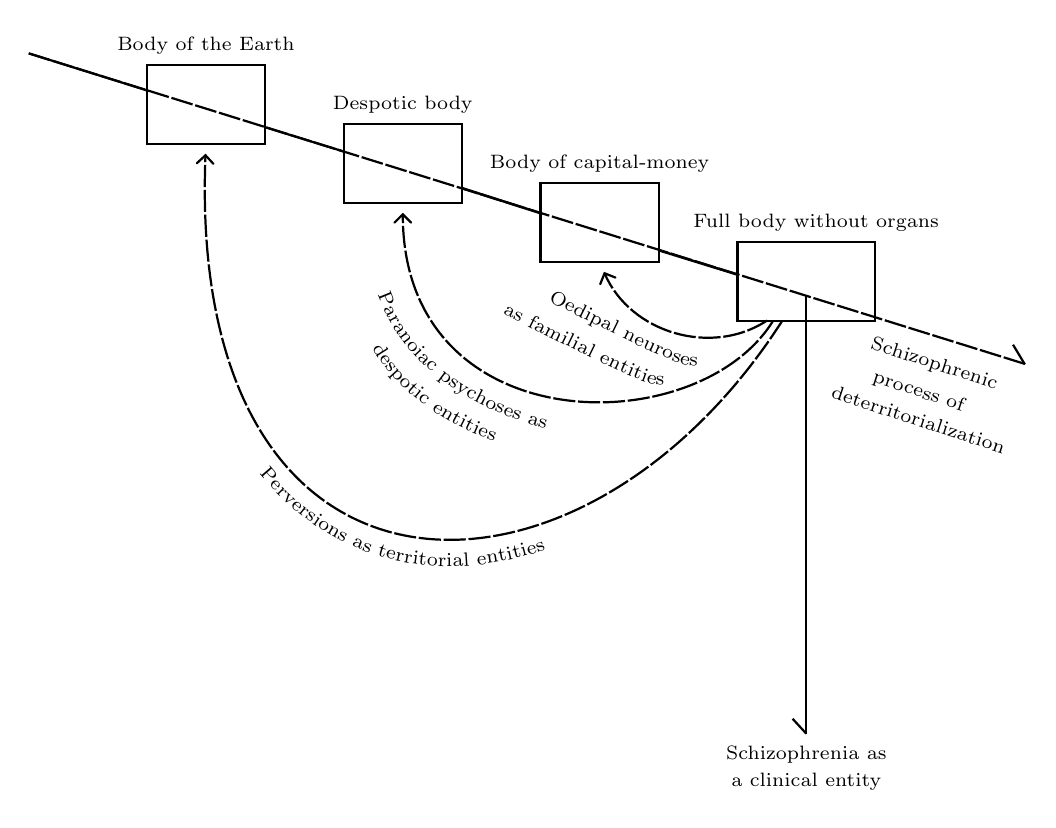
\begin{tikzpicture}
	%\draw[help lines] (0,0) grid (10,10);
	\draw[thick] (0,6) rectangle (1.5,5);
		\node (BE) at (0.75,5) {\textcolor{blue}{}};
	\draw[thick] (2.5,5.25) rectangle (4,4.25);
		\node (DB) at (3.25,4.25) {\textcolor{green}{}};
	\draw[thick] (5,4.5) rectangle (6.5,3.5);
		\node (BC) at (5.75,3.5) {\textcolor{red}{}};
	\draw[thick] (7.5,3.75) rectangle (9.25,2.75);
		\node (FE) at (8,2.84) {\textcolor{red}{}};
		\node (DE) at (8.03,2.88) {\textcolor{green}{}};
		\node (TE) at (8.15,2.88) {\textcolor{blue}{}};
	
	\node at (0.75,6.25) {{\scriptsize Body of the Earth}};
	\node at (3.25,5.5) {{\scriptsize Despotic body}};
	\node at (5.75,4.75) {{\scriptsize Body of capital-money}};
	\node at (8.5,4) {{\scriptsize Full body without organs}};
	
	%\def\myshift#1{\raisebox{-2.5ex}}
	\draw[-angle 90,thick, dash pattern={on 8pt off 1pt}] (FE) to[bend left=50] (BC);
	\draw [decorate, decoration={text along path, text align=center, text={|\scriptsize|Oedipal neuroses}}] (4.9,3.1) .. controls (6.9,2.1) .. (7.2,2.25);
	\draw [decorate, decoration={text along path, text align=center, text={|\scriptsize|as familial entities}}] (4.4,2.9) .. controls (6.4,1.9) .. (6.7,1.95);
	
	
	%\def\myshift#1{\raisebox{-2.5ex}}
	%\draw[thick,dashed,postaction={decorate,decoration={text along path,text align=center,text={|\sffamily\myshift|Paranoiac psychoses as}}}] (DB) .. controls (3.25,1.2) and (7,1.2) .. (DE);
	%before I had: to[bend left=100]
	%then I tried: to[out=247.5,in=270]
	
	
	\draw[-angle 90,thick,dash pattern={on 8pt off 1pt}] (DE) .. controls (7,1.2) and (3.25,1.2) .. (DB);
	\draw[decorate, decoration={text along path, text align=center, text={|\scriptsize|Paranoiac psychoses as}}] (3,5) .. controls (2,2) and (5,1) .. (7,1.25);	%(DB) -- (DE)
	\draw [decorate, decoration={text along path, text align=center, text={|\scriptsize|despotic entities}}] (2.75,4.7) .. controls (1.75,1.7) and (4.75,0.7) .. (6.75,1);
	
	
	%\def\myshift#1{\raisebox{-2.5ex}}
	%\draw[thick,dashed,postaction={decorate,decoration={text along path,text align=center, text={|\sffamily\myshift|Perversions as territorial entities}}}] (BE) .. controls (0.5,-1.25) and (5.5,-1.25) .. (TE);	
	%before I had: to[bend left=120]
	%then I tried: to[out=247.5,in=270]
	
	\draw[-angle 90,thick,dash pattern={on 8pt off 1pt}] (TE) .. controls (5.5,-1.25) and (0.5,-1.25) .. (BE);
	\draw [decorate, decoration={text along path, text align=center, text={|\scriptsize|Perversions as territorial entities}}] (0.25,4.65) .. controls (0.5,-1.6) and (5.5,-1.6) .. (8.15,2.4);
	
	\draw[thick, dash pattern={on 8pt off 1pt}] (-1.5,6.15) -- (11.17,2.2);	%diagonal line
	\node at (10,2.2) {\rotatebox{342}{\scriptsize{Schizophrenic}}};
	\node at (9.8,1.85) {\rotatebox{342}{\scriptsize{process of}}};
	\node at (9.8,1.5) {\rotatebox{342}{\scriptsize{deterritorialization}}};
	\draw[thick] (11.15,2.2) -- (11,2.45); %ugly-ass makeshift harpoon
	
	%filling in the diagonal line
	\draw[thick] (-1.5,6.15) -- (0,5.68);
	\draw[thick] (1.5,5.213) -- (2.5,4.903);
	\draw[line width=0.9] (4,4.44) -- (5,4.12);
	\draw[line width=0.9] (6.5,3.65) -- (7.5,3.34);
	
	%ugly-ass enlarged harpoon: decoration={markings,mark=at position 1 with {\arrow[scale=2,>=left to]{>}}},postaction={decorate}
	%for the enlarged harpoons, I'd be better off just drawing a line by hand
	
	\draw[thick] (8.375,3.08) -- (8.375,-2.5);	%vertical line
	\node at (8.375,-2.75) {{\scriptsize Schizophrenia as}};
	\node at (8.375,-3.1) {{\scriptsize a clinical entity}};
	%ugly-ass enlarged harpoon: decoration={markings,mark=at position 1 with {\arrow[scale=2,>=right to]{>}}},postaction={decorate}
	\draw[thick] (8.375,-2.49) -- (8.2,-2.3); %ugly-ass makeshift harpoon
	
	\end{tikzpicture}
		
	\vspace{0.5cm}
	
	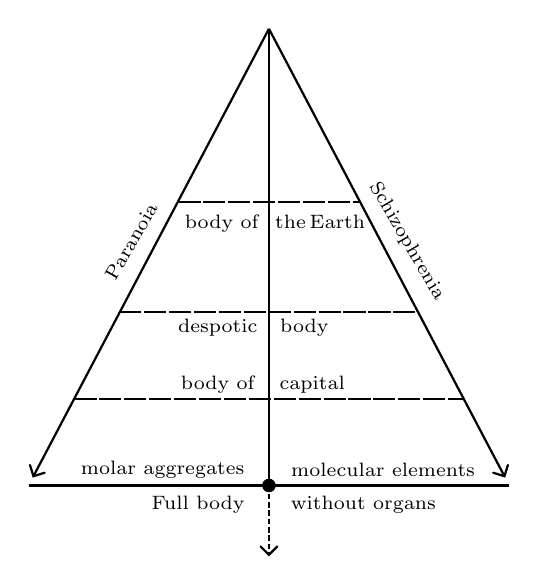
\begin{tikzpicture}
	%triangle
	\node[circle,draw=black, fill=black, inner sep=0pt,minimum size=4.5pt] (S) at (0,-0.1) {};
	\draw [-angle 90, thick]  	(0,5.7)--(-3,0);	%diagonal line
	\draw [-angle 90, thick]  	(0,5.7)--( 3,0);	%diagonal line
	\draw [thick]  	  (-3.05,-0.1)--(3.05,-0.1);	%horizontal line
	\draw [thick]  				(0,5.7)--(0,-0.1);	%vertical line
	\draw [-angle 90,thick,dash pattern={on 2pt off 1pt}]  (0,-0.1)--(0,-1);	%vertical arrow
	
	%horizontal dashed lines
	\draw[thick, dash pattern={on 8pt off 1pt}] (-1.15,3.5)--(1.15,3.5);		%top dashed line
	\draw[thick, dash pattern={on 8pt off 1pt}] (-1.9,2.1)--(1.9,2.1);	%mid dashed line
	\draw[thick, dash pattern={on 8pt off 1pt}] (-2.47,1)--(2.48,1);		%bottom dashed line
	
	%labels
	\node at (-0.6,3.22) {{\scriptsize body of}};
	\node at ( 0.65,3.25) {{\scriptsize the$\,$Earth}};
	%
	\node at (-0.65,1.9) {{\scriptsize despotic}};
	\node at (0.45,1.9) {{\scriptsize body}};
	%
	\node at (-0.65,1.18) {{\scriptsize body of}};
	\node at (0.55,1.18) {{\scriptsize capital}};
	%
	\node at (-1.35,0.1) {{\scriptsize molar aggregates}};
	\node at (1.45,0.1) {{\scriptsize molecular elements}};
	%
	\node at (-0.9,-0.35) {{\scriptsize Full body}};
	\node at ( 1.2,-0.35) {{\scriptsize without organs}};
	
	%diagonal labels
	\node at (-1.75,3) {\rotatebox{60}{\text{{\scriptsize Paranoia}}}};
	\node at ( 1.75,3) {\rotatebox{300}{\text{{\scriptsize Schizophrenia}}}};
	
	\end{tikzpicture}
	
		
\end{document}